\documentclass{webofc}
\usepackage[varg]{txfonts}   % Web of Conferences font
%
% Put here some packages required or/and some personnal commands
%
\usepackage{hyperref}
\hypersetup{colorlinks=false}

%
\begin{document}
%
\title{IPv6-only networking on WLCG}
%
% subtitle is optionnal
%
%%%\subtitle{Do you have a subtitle?\\ If so, write it here}

\author{
  \firstname{Marian} \lastname{Babik}\inst{1}\and
  \firstname{Martin} \lastname{Bly}\inst{2}\and
  \firstname{Tim} \lastname{Chown}\inst{3}\and
  \firstname{Dimitrios} \lastname{Christidis}\inst{4}\and
  \firstname{Ji\v{r}i} \lastname{Chudoba}\inst{5}\and
  \firstname{Catalin} \lastname{Condurache}\inst{6}\and
  \firstname{Thomas} \lastname{Finnern}\inst{7}\and
  \firstname{Terry} \lastname{Froy}\inst{8}\and
  \firstname{Costin} \lastname{Grigoras}\inst{1}\and
  \firstname{Kashif} \lastname{Hafeez}\inst{2}\and
  \firstname{Bruno} \lastname{Hoeft}\inst{9}\and
  \firstname{David P.} \lastname{Kelsey}\inst{2}\thanks{\email{david.kelsey@stfc.ac.uk}} \and
  \firstname{Raul} \lastname{Lopes} \inst{10} \and
  \firstname{Fernando} \lastname{L\'opez~Mu\~noz}\inst{11,12}\fnsep\and
  \firstname{Edoardo} \lastname{Martelli}\inst{1}\and
  \firstname{Raja} \lastname{Nandakumar}\inst{2}\and
  \firstname{Kars} \lastname{Ohrenberg}\inst{7}\and
  \firstname{Francesco} \lastname{Prelz}\inst{13}\and
  \firstname{Duncan} \lastname{Rand}\inst{14}\and
  \firstname{Andrea} \lastname{Sciab\`a}\inst{1}
}

\institute{ 
  European Organization for Nuclear Research (CERN), CH-1211 Geneva 23, Switzerland
\and
  UKRI STFC Rutherford Appleton Laboratory, Harwell Campus, Didcot, Oxfordshire OX11 0QX, United Kingdom
\and
  JISC, Lumen House, Library Avenue, Harwell Campus, Didcot, Oxfordshire OX11 0SG, United Kingdom
\and
  University of Texas at Arlington, Arlington TX, United States of America
\and
  Institute of Physics, Academy of Sciences of the Czech Republic, Na Slovance 2 182 21 Prague 8, Czech Republic
\and
  EGI Foundation, Science Park 140, 1098 XG Amsterdam, The Netherlands
\and
  Deutsches Elektronen-Synchrotron DESY, Notkestra\ss e 85, D-22607 Hamburg, Germany
\and
  Queen Mary University of London, Mile End Road, London E1 4NS, United Kingdom
\and
  Karlsruhe Institute of Technology, Hermann-von-Helmholtz-Platz 1, D-76344 Eggenst.-Leopoldsh., Germany 
\and
 College of Engineering, Design and Physical Sciences, Brunel University London, Uxbridge, UB8 3PH, United Kingdom 
\and
  Port d'Informaci\'o Cient\'ifica, Campus UAB, Edifici D, E-08193 Bellaterra, Spain
\and
  Centro de Investigaciones Energ\'eticas, Medioambientales y Tecnol\'ogicas (CIEMAT), Madrid, Spain
\and
  INFN, Sezione di Milano, via G. Celoria 16, I-20133 Milano, Italy
\and
  Imperial College London, South Kensington Campus, London SW7 2AZ, United Kingdom
          }

\abstract{


The use of IPv6 on the general internet continues to grow.
The transition of the Worldwide Large Hadron Collider Computing Grid 
(WLCG) central and storage services to dual-stack IPv4/IPv6 is progressing well,
thus enabling the use of IPv6-only CPU resources as agreed by the WLCG
Management Board and presented by us at earlier CHEP conferences.
During the last year, the HEPiX IPv6 working group has continued to chase
and support the transition to dual-stack services.
We present the status of the transition and some tests that have been made of IPv6-only CPU
showing the successful use of IPv6 protocols in accessing WLCG services.
The dual-stack deployment does however result in a networking environment
which is much more complex than when using just IPv6. The group is investigating the removal of the IPv4 protocol in
places. We present the areas where this could be useful together with our future plans.
}
%
\maketitle
%
\section{Introduction}
\label{sec-intro}
%section 1

The HEPiX IPv6 Working Group \cite{ipv6wg} has been investigating the many issues involved in the deployment and use of
IPv6 in HEP in general and more specifically in WLCG. The group's paper at CHEP2016 \cite{ipv6chep2016}
presented the status then of the work to allow sites to deploy IPv6-only CPU resources. Driven by the
requirements of the LHC experiments, the WLCG Management Board, in September 2016, had approved our plan
that all WLCG Tier-2 storage services should aim to support dual-stack IPv6/IPv4 by the end of 2018. Since then the
group has worked with others to encourage, support and monitor that transition and to identify and help
solve any technical issues as they arise.

%This paper is organised as follows.  Section 2 presents the current status of the transition for the Tier0/Tier1s, the Tier2s and the Experiment Services.
%Section 3 presents an update on service availability and network monitoring and also reports on the fraction of FTS data transfers currently taking place over IPv6.
%Finally section 4 contains future plans and conclusions. 

 


\section{Status of the transition to dual-stack storage}
\label{sec-trans}
%section 2 Status of the transition to dual-stack storage
% sub-section a) Tier 0 and Tier 1's  (Bruno)
% sub-section b) Tier 2's  (Andrea)
% sub-section c) LHCOPN & LHCONE  (Bruno)
% sub-section d) WLCG Data Transfers (Dave)

% Do we start with a few general words of introduction about the general aims and history of the transition to dual-stack storage?
% Together with reminders of the agreed timetable (and refer to old CHEP papers from our group)?

The long process of enabling the protocol IPv6 at LHC started already 10 years ago in 2010. Today, after extensive testing by the HEPiX IPv6 working group and the strong support of the storage developer community, the current WLCG storage and grid-middleware applications now fully support the use of IPv4 and IPv6 protocols simultaneously; they are dual-stack ready or even protocol agnostic.


% Subsection '2a'
% Tier 0 and Tier 1's
%
%\subsection{Deployment at the Tier-0 and Tier-1 sites}
\subsection{Deployment at Tier-0 and Tier-1's}
After the aforementioned ten years the storage environment is almost completely dual-stack ready. At the CERN WLCG Tier-0 and at the 14 Tier-1s, dual-stack IPv6/IPv4 is nearly fully enabled. Only the Tier-1 site at the Kurchatov Institute in Moscow, part of the Russian Federation, is still currently running on IPv4-only. This enables a total of 96\% of the Tier-1 storage of WLCG to be accessible via IPv6 as shown in table~\ref{tab:t012stor}.
\begin{table}[h]
\centering
\caption{Fraction of Tier-1 and Tier-2 storage available over IPv6}
\label{tab:t012stor}
\begin{tabular}{lccccc}
\hline
& ALICE & ATLAS & CMS & LHCb & Global \\\hline
Tier-1 storage & 78\% & 96\% & 100\% & 94\% & 96\% \\
Tier-2 storage & 86\% & 59\% &  89\% & 75\% & 74\% \\\hline
\end{tabular}
\end{table}

The FTS server at FNAL is still currently running in IPv4 preferred mode. There was a long-standing malfunctioned transfer issue to IPv4-only Tier-2 sites in the USA which is now solved. This last server will be deployed in dual-stack in the near future.

\subsection{Deployment at Tier-2 sites}
The deployment of IPv6 at Tier-2 sites is still proceeding even after the
official deadline expired at the end of 2018. It was decided not to
give the deadline a formal extension, but just to encourage all
remaining sites to complete the IPv6 deployment ``as soon as
possible'': the main motivations were that \emph{a)} sites behind
schedule were encountering objective difficulties and \emph{b)} the
most effective deadline would be imposed by the experiments
themselves, if they wished, for example, to require IPv6 for
production. This choice was confirmed by the steady progress observed
during 2019, as it can be seen in figure~\ref{fig:t2depl}.
\begin{figure}[h]
\centering
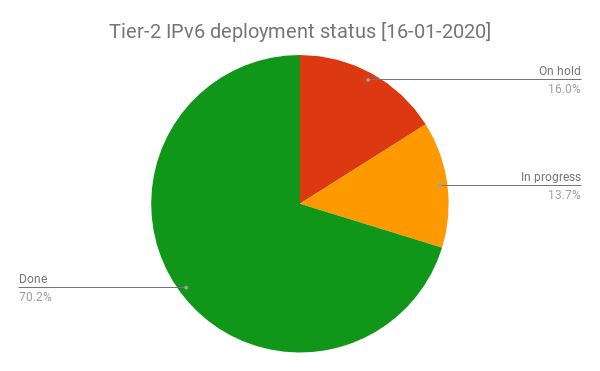
\includegraphics[width=6cm]{chart2}
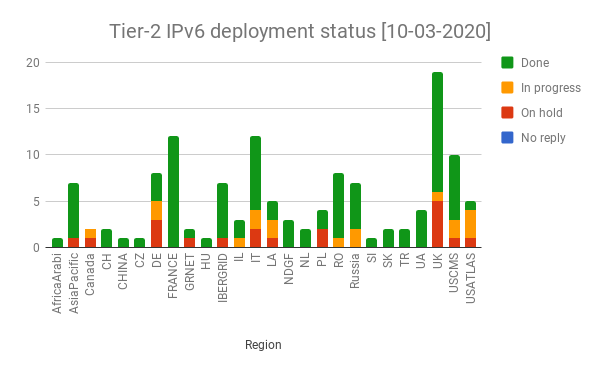
\includegraphics[width=6cm]{chart}
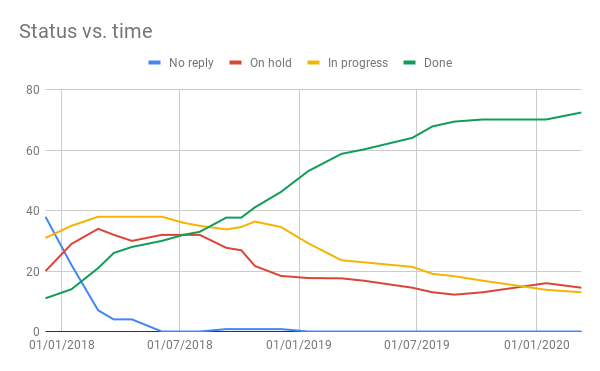
\includegraphics[width=6cm]{chart3}
\caption{(left) Tier-2 deployment status by site globally, (right) by region, and (bottom) time evolution}
\label{fig:t2depl}
\end{figure}

The time evolution of the site status shows a steady increase of the
number of sites that have deployed IPv6, until a more recent
slowdown. This is consistent with the hypothesis that the remaining
sites are those facing the biggest difficulties. A detailed analysis
of the tickets shows that, in many cases, sites need to wait for the
IPv6 deployment on site, which often depends on people different from
the WLCG site staff. The fraction of the Tier-2 storage that is
accessible via IPv6 is shown in table~\ref{tab:t12stor} for each
experiment, and significant differences are apparent.
\begin{table}[h]
\centering
\caption{Fraction of Tier-1 and Tier-2 storage available over IPv6}
\label{tab:t12stor}
\begin{tabular}{lccccc}
\hline
& ALICE & ATLAS & CMS & LHCb & Global \\\hline
Tier-1 storage & 78\% & 96\% & 100\% & 94\% & 96\% \\ 
Tier-2 storage & 86\% & 59\% &  89\% & 75\% & 74\% \\\hline
\end{tabular}
\end{table}
Two experiments (ALICE and CMS) are very close to having all their
Tier-2 storage on IPv6, LHCb has little Tier-2 storage to begin with
due to their particular computing model and ATLAS is getting better,
but still far from the goal.


\subsection{LHCOPN and LHCONE}

The LHCOPN and LHCONE are both virtual private networks (VPN) serving the Large Hadron Colider Experiments. Both networks are from the end of 2016 onward dual-stack ready. LHCOPN is a CERN (Tier-0) centric star network mainly deployed for the distribution of the raw detector data to the Tier-1 sites. Since the majority of Tier-1 sites are dual-stack ready and even while the protocol IPv6 is preferred it is still not the situation that IPv6 is the only transfer protocol, but a tendency towards IPv6 file transfers are recognizable. LHCONE is a network of close to 140 sites connected trough Virtual Routing and Forwarding implementations at 26 different network service providers (NSP). All connected end sites deploying a Border Gateway Protocol (BGP) routing table and advertising their own Classless Inter-Domain Routing (CIDR) to the connecting NSP. The network itself is already since long IPv6 ready. The connected end sites are becoming more and more IPv6 ready. This is recognizable at the  transfer protocol changes from IPv4 towards IPv6. The high usage of the IPv4 transfer protocol visualizes that the fraction of IPv4 only sites is still quite substantial.

%section{File Transfers

\subsection{File transfers}

Over the last 2 years we have been regularly tracking the fraction of WLCG file transfers that take place over IPv6.
(needs more description).

The fraction of data transfers over FTS on IPv6 as a function of date is shown in  figure~\ref{fig:FTS}.
\begin{figure}[h]
\centering
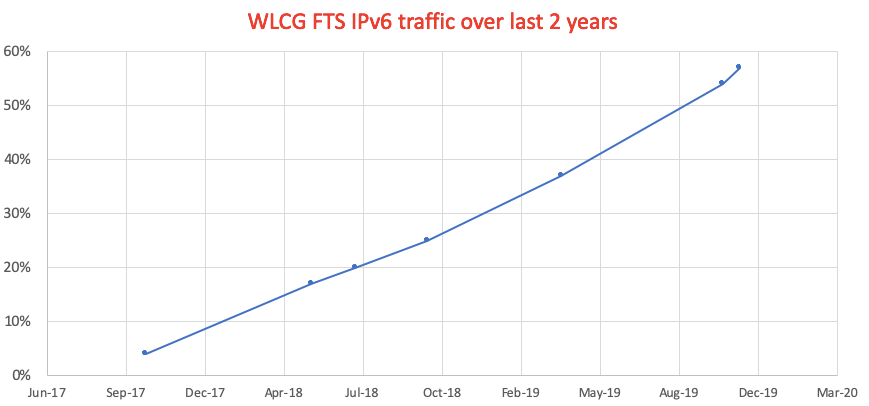
\includegraphics[width=10cm]{FTS}
\caption{Percentage of FTS data transfers over IPv6}
\label{fig:FTS}
\end{figure}


%% Subsection '2a'
% Tier 0 and Tier 1's
%
Some efforts were made to investigate whether the WLCG software packages could be enabled to run in a dual-stack environment or even become protocol agnostic. The first software packages that were examined were data transfer software packages like FTS and SRM. After the examination some software packages were replaced like AFS with EOS, or CASTOR with DPM. Today the storage environment is dual/stack ready and at CERN the Tier-0 is IPv6 and IPv4 dual-stack is enabled. The Tier-1 sites: CA-Triumf, DE-KIT, ES-PIC, FR-CCIN2P3, IT-INFN-CNAF, NDGF, NL-T1 (SARA-Matrix and NIKHEF), RRC-JINR-T1, TW-ASGC, UK-T1-RAL, US-T1-BNL, US-T1-FNAL are dual-stack deployed as shown in the following figure. ~\ref{fig:t1ds}.
\begin{figure}[t]
\centering
%\includegraphics[width=13cm]{Tier-1-IPv6-dual-stack}
\includegraphics[width=13cm]hepix-ipv6-tier01-dual-stack.png}
%\includegraphics[width=13cm]{t1ds}
\caption{Tier-0/1 IPv4/6 dual-stack redyness incl dual-stack perfsonar server deployment}
\label{fig:t1ds}
\end{figure}

But even while the IPv6 redeaness deadline in April 2018 is long ago, there is one part of the russian Tier-1 RRC-KI-T1 still deployed with IPv4 only. The dual-stack perfsonar server is deployed at almost all sites except NL-T1-NIKHEF and RRC-KI-T1. The FTS server at FNAL is still running in IPv4 prefered mode. There were a long standing malfunctioned transfer issue to IPv4 only US-Tier-2 sites which is solved now. This last server will get deployed in dual-stack as soon as possible.   

%\subsection{Deployment at Tier-2 sites}
The deployment of IPv6 at Tier-2 sites is still proceeding even after the
official deadline expired at the end of 2018. It was decided not to
give the deadline a formal extension, but just to encourage all
remaining sites to complete the IPv6 deployment ``as soon as
possible'': the main motivations were that \emph{a)} sites behind
schedule were encountering objective difficulties and \emph{b)} the
most effective deadline would be imposed by the experiments
themselves, if they wished, for example, to require IPv6 for
production. This choice was confirmed by the steady progress observed
during 2019, as it can be seen in figure~\ref{fig:t2depl}.
\begin{figure}[h]
\centering
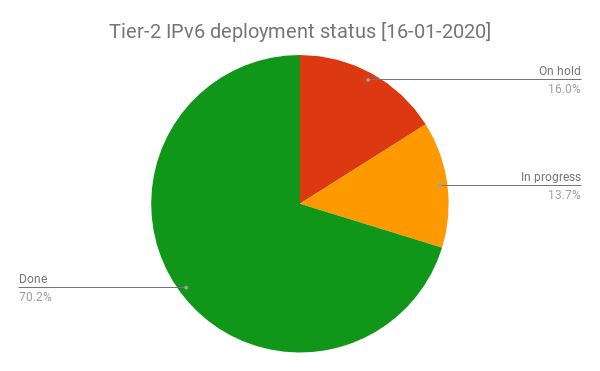
\includegraphics[width=6cm]{chart2}
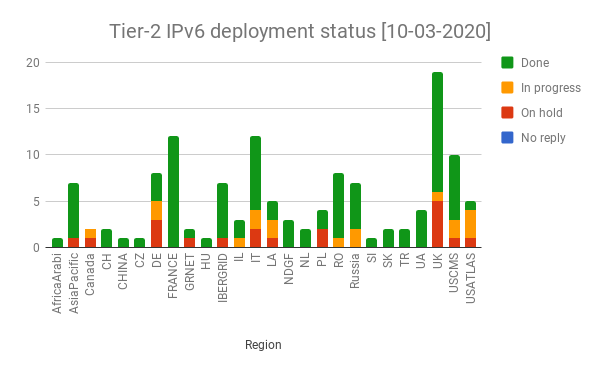
\includegraphics[width=6cm]{chart}
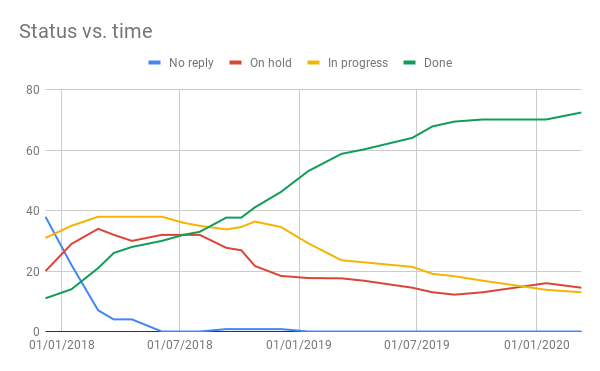
\includegraphics[width=6cm]{chart3}
\caption{(left) Tier-2 deployment status by site globally, (right) by region, and (bottom) time evolution}
\label{fig:t2depl}
\end{figure}

The time evolution of the site status shows a steady increase of the
number of sites that have deployed IPv6, until a more recent
slowdown. This is consistent with the hypothesis that the remaining
sites are those facing the biggest difficulties. A detailed analysis
of the tickets shows that, in many cases, sites need to wait for the
IPv6 deployment on site, which often depends on people different from
the WLCG site staff. The fraction of the Tier-2 storage that is
accessible via IPv6 is shown in table~\ref{tab:t12stor} for each
experiment, and significant differences are apparent.
\begin{table}[h]
\centering
\caption{Fraction of Tier-1 and Tier-2 storage available over IPv6}
\label{tab:t12stor}
\begin{tabular}{lccccc}
\hline
& ALICE & ATLAS & CMS & LHCb & Global \\\hline
Tier-1 storage & 78\% & 96\% & 100\% & 94\% & 96\% \\ 
Tier-2 storage & 86\% & 59\% &  89\% & 75\% & 74\% \\\hline
\end{tabular}
\end{table}
Two experiments (ALICE and CMS) are very close to having all their
Tier-2 storage on IPv6, LHCb has little Tier-2 storage to begin with
due to their particular computing model and ATLAS is getting better,
but still far from the goal.


%\subsection{LHCOPN and LHCONE}

The LHCOPN and LHCONE are both virtual private networks (VPN) serving the Large Hadron Colider Experiments. Both networks are from the end of 2016 onward dual-stack ready. LHCOPN is a CERN (Tier-0) centric star network mainly deployed for the distribution of the raw detector data to the Tier-1 sites. Since the majority of Tier-1 sites are dual-stack ready and even while the protocol IPv6 is preferred it is still not the situation that IPv6 is the only transfer protocol, but a tendency towards IPv6 file transfers are recognizable. LHCONE is a network of close to 140 sites connected trough Virtual Routing and Forwarding implementations at 26 different network service providers (NSP). All connected end sites deploying a Border Gateway Protocol (BGP) routing table and advertising their own Classless Inter-Domain Routing (CIDR) to the connecting NSP. The network itself is already since long IPv6 ready. The connected end sites are becoming more and more IPv6 ready. This is recognizable at the  transfer protocol changes from IPv4 towards IPv6. The high usage of the IPv4 transfer protocol visualizes that the fraction of IPv4 only sites is still quite substantial.




\section{IPv6-only networking}
\label{sec-onlysix}
% section 3 IPv6-only networking
% sub-section a) Aims of moving to IPv6-only and issues to be tackled  (Francesco)
% sub-section b) The case for an IPv6-only LHCOPN  (Edoardo)
% sub-section c) Testing of IPv6-only (Raul Lopes - Brunel)
% sub-section d) Future plans (Francesco)

A few years ago, RFC 6586 (\cite{rfc}) reported on a survey on IPv6-only
networking for mainstream applications (gaming, telephony,
multimedia, etc.) and observed that {\it \guillemotleft it is possible to employ IPv6-only
networking\guillemotright} and that {\it \guillemotleft for large classes of applications
there are no downsides or the downsides are negligible\guillemotright}.
This, along with the good working relations we established over
the past years with the HEP software stack developers,
encouraged us to test 
scenarios where the transient complication of running and managing
two independent network stacks is eventually over and we are `back' to just
running IPv6.

\subsection{Aims of moving to IPv6-only and issues to be tackled}
\label{ssec:ipv6onlymove}
A dual-stack IPv6/IPv4 setup includes many components and services that need
to be deployed twice {\it and kept in sync}: firewall rules and access
lists, address assignment services, routing rules, network monitoring,
diagnostics and
intrusion detection infrastructures - just to name a few.
Removing this duplication is highly desirable both for better maintainability
and cost-saving.
However, this {\it requires} a technical
solution to access any site and service that may remain accessible via IPv4
{\it only}.
This trailing remainder of sites will be hopefully
shrinking but will likely exist for a very long time (see
e.g. \cite{ipv6trans} and references therein).
It is actually expected that after large blocks of public IPv4
addresses start being returned to the market, their market price will
decrease and offset any economic drive connected to the IPv4 address shortage,
{\it relieving} the pressure for migration.\par

The standard solution for accessing IPV4-only services from an IPv6-only
network is the deployment of DNS64 (RFC6147) and stateful
NAT64 (RFC6146 \cite{rfc}) services. DNS64 maps names that are resolved to
an IPv4 address only ('{\tt A}' records) to a synthesized IPv6 address composed
of a default prefix\footnote{Usually {\tt 64:ff9b::}.} plus the four bytes of
the IPv4 address. Traffic towards the DNS64 prefix is then routed to
a NAT64 service attached to the public IPv4 network. This will in turn map the
source ports, translate the IP packets to IPv4 and convert any return traffic
back to IPv6. While NAT64 and DNS64 services start being incorporated by
several technology developers (especially in the 'carrier-grade' NAT 
appliance market),
just a few open-source reference implementations exist for UNIX, with
JOOL\footnote{\tt https://www.jool.mx} apparently being the only one 
under active development.\par

While IPv6-only environments can present a few operational challenges that
can be worked around\footnote{Some OS-specific network management tools,
firewall appliances and network monitoring and diagnostic tools were found
to be defective or immature, see RFC 6586 \cite{rfc} for details.},
one-step (6$\rightarrow$4) address translation techniques do and will fail whenever 
IPv4 literal addresses are explicitely handled, stored or signaled by
network applications or protocols. We feel that the time is ripe to
start identifying this class of applications and protocols and direct an early effort
at cleaning them of {\it any} usage or reference to IPv4 literals. While 
two-step (4$\rightarrow$6$\rightarrow$4) address translation techniques
such as XLAT464\footnote{See RFC 6877 \cite{rfc}. XLAT464 keeps a private
IPv4 address assigned to devices connected to IPv6-only networks and
performs an additional address translation at the device level.}
are currently being added to 
network stacks especially at the request of telephony carriers that operate
IPv6-only networks, we see this extra indirection as an (inefficient)
workaround that just hides issues that should be fixed at the application
level. Locating this issues as early as possible motivates the experimental
operation of typical
WLCG sites with IPv6-only networking and NAT64/DNS64, as described
later (\S \ref{ssec:ipv6onlytest}).

\subsection{The case for an IPv6-only LHCOPN}
\input subsection-3b-lhcopn.tex

\subsection{Testing of IPv6-only}
\label{ssec:ipv6onlytest}
\input subsection-3c-ipv6only-testing.tex

\subsection{Future plans}
Insufficiently tested or immature code and the requirement that IPv6-based
tools and infrastructures perform at least equally well as their IPv4
counterparts have been the opposite, conflicting poles of every IPv6
deployment effort so far. This continues to be true in the process
of completing the transition. We therefore keep considering
testing activities (and the consequent early detection of further application
development needs), as a value that our group can provide. So we plan
to increase the number of sites and stakeholders involved in testing IPv6-only 
scenarios. The aim is to stress-test existing networking software components
that implement any needed transition protocol (especially NAT64 and DNS64, as 
their implementations under current maintenance are rare) and detect
residual uses of IPv4 literals or IPv4-specific APIs in both applications and
network protocols as early as possible.\par
Any use of IPv4 that cannot respond properly to a NAT64-mediated
transaction
\footnote{More complex and inefficient address
translation solutions such as the deployment of 'customer'-side address
translation for RFC 6877 (\cite{rfc}) 424XLAT should be
seen as options of last resort, see \S \ref{ssec:ipv6onlymove} above.}
should be seen as an issue to be reported, tracked and eventually
addressed by developers: we plan to deal with these just as we did
with the lack of IPv6 support or the incorrect address selection
strategies we were able to identify so far.


\section{Conclusions and future plans}
\label{sec-concl}
% section 4 Conclusions (Dave)
%\subsection{Future plans}

We have presented the status of the WLCG transition to the use of dual-stack IPv6/IPv4. The Tier-1 transition is nearly complete and 
more than 70\% of the Tier-2 storage is available over IPv6. The transition will only be completed once we remove the complexity of
dual-stack networking and the WLCG core infrastructure is IPv6-only.


Insufficiently tested or immature code and the requirement that IPv6-based
tools and infrastructures perform at least equally well as their IPv4
counterparts have been the opposite, conflicting poles of every IPv6
deployment effort so far. This continues to be true in the process
of completing the WLCG transition. We conclude that
testing activities, and the consequent early detection of further application
development needs, will keep the working group busy. We plan
to increase the number of sites and stakeholders involved in testing IPv6-only 
scenarios. The aim is to stress-test existing networking software components
that implement any needed transition protocol (especially NAT64 and DNS64, as 
their implementations under current maintenance are rare) and detect
residual uses of IPv4 literals or IPv4-specific APIs in both applications and
network protocols as early as possible.\par
Any use of IPv4 that cannot respond properly to a NAT64-mediated
transaction\footnote{More complex and inefficient address
translation solutions such as the deployment of `customer'-side address
translation for RFC 6877 \cite{rfc} 464XLAT or RFC 7597/9 \cite{rfc} MAP-E/T  should be
seen as options of last resort, see \S \ref{ssec:ipv6onlymove} above.}
should be seen as an issue to be reported, tracked and
addressed by developers: we plan to deal with these just as we did
with the lack of IPv6 support or the incorrect address selection
strategies we were able to identify so far.\par
Once we are confident that IPv6-only scenarios work well and that
all issues found with the use of transition protocols have been fixed, we will
propose a timetable for the deployment of an IPv6-only networking 
environment for WLCG.


% Etc. etc. etc.

%For one-column wide figures use syntax of figure~\ref{fig-1}
%\begin{figure}[h]
%% Use the relevant command for your figure-insertion program
%% to insert the figure file.
%\centering
%\includegraphics[width=1cm,clip]{tiger}
%\caption{Please write your figure caption here}
%\label{fig-1}       % Give a unique label
%\end{figure}
%
%For two-column wide figures use syntax of figure~\ref{fig-2}
%\begin{figure*}
%\centering
%% Use the relevant command for your figure-insertion program
%% to insert the figure file. See example above.
%% If not, use
%\vspace*{5cm}       % Give the correct figure height in cm
%\caption{Please write your figure caption here}
%\label{fig-2}       % Give a unique label
%\end{figure*}
%
%For figure with sidecaption legend use syntax of figure
%\begin{figure}
%% Use the relevant command for your figure-insertion program
%% to insert the figure file.
%\centering
%\sidecaption
%\includegraphics[width=5cm,clip]{tiger}
%\caption{Please write your figure caption here}
%\label{fig-3}       % Give a unique label
%\end{figure}
%
%For tables use syntax in table~\ref{tab-1}.
%\begin{table}
%\centering
%\caption{Please write your table caption here}
%\label{tab-1}       % Give a unique label
%% For LaTeX tables you can use
%\begin{tabular}{lll}
%\hline
%first & second & third  \\\hline
%number & number & number \\
%number & number & number \\\hline
%\end{tabular}
%% Or use
%\vspace*{5cm}  % with the correct table height
%\end{table}
%
% BibTeX or Biber users please use (the style is already called in the class, ensure that the "woc.bst" style is in your local directory)
% \bibliography{name or your bibliography database}
%
% Non-BibTeX users please use
%
%\begin{thebibliography}{}
%
% and use \bibitem to create references.
%
%\bibitem{rfc} All Internet Engineering Task Force Requests For Comments (RFC) do
%cuments are available
%from URLs such as http://www.ietf.org/rfc/rfcNNNN.txt where NNNN is the RFC numb
%er, for example {\tt http://www.ietf.org/rfc/rfc2460.txt}
% Format for Journal Reference
%Journal Author, Journal \textbf{Volume}, page numbers (year)
% Format for books
%\bibitem{RefB}
%Book Author, \textit{Book title} (Publisher, place, year) page numbers
% etc
%\end{thebibliography}

\section {The References need updating} 
These are from the CHEP2018 paper!

\begin{thebibliography}{}
%
% and use \bibitem to create references.
%
% Format for Journal Reference
%Journal Author, Journal \textbf{Volume}, page numbers (year)
% Format for books
%\bibitem{RefB}
%Book Author, \textit{Book title} (Publisher, place, year) page numbers
% etc


%section 1 references
%\bibitem{ipv6wg} The HEPiX IPv6 Working Group, http://hepix-ipv6.web.cern.ch
\bibitem{ipv6wg}
S. Campana et al, J. Phys. Conf. Ser. {\bf513}, 062026 (2014)



%\bibitem{ipv6chep2016} 
% M. Babik et al, J. Phys. Conf. Ser. {\bf898}, 082033 (2017)
\bibitem{ipv6chep2018} 
M. Babik et al, J. Phys. Conf. Ser. {\bf214}, 08010 (2019)

\bibitem{eos} A. J. Peters et al, J. Phys. Conf. Ser. {\bf664}, 042042 (2015)


%section 2 references

\bibitem{rfc} 
All Internet Engineering Task Force Requests For Comments (RFC) documents are available
from URLs such as https://www.ietf.org/rfc/rfcNNNN.txt where NNNN is the RFC number, for example {\tt https://www.ietf.org/rfc/rfc2460.txt}



%section 2 intro para

\bibitem{ipv6chep2015} 
J. Bernier et al, J. Phys. Conf. Ser. {\bf664}, 052018 (2015)

%section 2.1 Tier 0/1
\bibitem{fts3}
A.~A. Ayllon et al, 
%M~Salichos, M~K Simon, and O~Keeble.
%\newblock Fts3: New data movement service for wlcg.
J. Phys. Conf. Ser. {\bf 513}, 032081 (2014)

%section 2.2 Tier 2

%section 2.3 LHCOPN
\bibitem{opnone}
E. Martelli et al, J. Phys. Conf. Ser. {\bf 664}, 052025 (2015)

%section 2.4 Data transfers



%section 2 Experiments
%\bibitem{alien} 
%S. Bagnasco et al, J. Phys. Conf. Ser. {\bf119(6)}, 062012 (2008)

%\bibitem{xrootd}
%L. Bauerdick et al, J. Phys. Conf. Ser. {\bf 396} 042009 (2012)

%\bibitem{jalien}
%A. Grigora et al, J. Phys. Conf. Ser. {\bf523}, 012010 (2014)

%\bibitem{glideinwms} 
%http://iopscience.iop.org/article/10.1088/1742-6596/119/6/062044
%I. Sfiligoi, J. Phys. Conf. Ser. {\bf119(6)}, 062044 (2008)

%\bibitem{htcondor}
%D. Thain et al, Concurrency - Practice and Experience, {\bf 7(2-4)}, 323 (2005)

%\bibitem{dirac} A. Tsaregorodtsev et al, J. Phys. Conf. Ser. {\bf513}, 032096 (2014)

%LHCb : LHCb collaboration, A. A. Alves Jr. et al., The LHCb detector at the LHC, JINST 3 (2008) S08005

%section 3 references

%section 3.1
\bibitem{ipv6trans}
M. Nikkhah and R. Gu\'erin, 
IEEE/ACM Transactions on Networking, {\bf 24(4)}, 2291 (2016)

\bibitem{jool}
https://www.jool.mx

%section 3.2

\bibitem{RefLHCOPNEv4v6}
LHCOPN and LHCONE traffic flows on the CERN border routers, 
https://twiki.cern.ch/twiki/bin/view/LHCOPN/LHCOPNEv4v6Traffic


%section 3.3
\bibitem{frontier}
http://frontier.cern.ch/

%\bibitem{sam}
%A. Aimar et al, J. Phys. Conf. Ser. {\bf 898(9)}, 092033 (2017)
%A~Aguado Corman, P~Andrade, S~Belov, J~Delgado Fernandez, B~Garrido Bear, M~Georgiou, E~Karavakis, L~Magnoni, R~Rama Ballesteros, H~Riahi, J~Rodriguez Martinez, P~Saiz, and D~Zolnai.
%\newblock Unified monitoring architecture for it and grid services.


%\bibitem{etf}
%Marian Babik, CERN,
%\newblock Experiments {Test} {Framework} ({ETF}).
%http://etf.cern.ch/docs/latest/

%\bibitem{perfsonar} 
%A. Hanemann et al, 
%Jeff~W. Boote, Eric~L. Boyd, J{\'e}r{\^o}me Durand, Loukik
 %Kudarimoti, Roman {\L}apacz, D.~Martin Swany, Szymon Trocha, and Jason Zurawski.
%\newblock Perfsonar: A service oriented architecture for multi-domain network monitoring.
%\newblock In Boualem Benatallah, Fabio Casati, and Paolo Traverso, editors,
  %{\em Service-Oriented Computing - ICSOC 2005}, pages 241--254, Berlin, Heidelberg, 2005. Springer Berlin Heidelberg.

%\bibitem{wlcg-NTWG}
%S.~McKee et al, J. Phys. Conf. Ser. {\bf 664(5)} 052003 (2015)
%S.~Campana, A.~Di Girolamo, T.~Wildish, J.~Closier, S.~Roiser, C.~Grigoras, I.~Vukotic, M.~Salichos, Kaushik De, V.~Garonne, J.A.D. Cruz, A.~Forti, C.J. Walker, D.~Rand, A.~de~Salvo, E.~Mazzoni, I.~Gable, F.~Chollet, L.~Caillat, F.~Schaer, Hsin-Yen Chen, U.~Tigerstedt, G.~Duckeck, B.~Hoeft, A.~Petzold, F.~Lopez, J.~Flix, S.~Stancu, J.~Shade, M.~O'Connor, V.~Kotlyar, and J.~Zurawski.
%\newblock Integrating network and transfer metrics to optimize transfer efficiency and experiment workflows.


%\bibitem{psmad}  
%perfSONAR Consortium,
%\newblock {perfSONAR} {Monitoring and Debugging Dashboard (MADDASH)}.
%http://psmad.grid.iu.edu/toolkit/
%http://psmad.grid.iu.edu/maddash-webui/
%index.cgi?dashboard=OPN%20Mesh%20Config

%\bibitem{grafana-ipv6}
%CERN monitoring team,
%\newblock {CERN} {MONIT} {Grafana} {Dashboard}.
%https://monit-grafana.cern.ch/





%\bibitem{RefLHCOPNEv4v6}
%LHCOPN and LHCONE traffic flows on the CERN border routers, 
%https://twiki.cern.ch/twiki/bin/view/LHCOPN/LHCOPNEv4v6Traffic


%\bibitem{grafana-FTS}
%CERN~{MONIT} team.
%\newblock {CERN} {MONIT} {Grafana} {FTS} {Dashboard}.
 
%\bibitem{grafana-WLCG-Transfers}
%CERN~{MONIT} team.
%\newblock {CERN} {MONIT} {Grafana} {WLCG} {Transfers} {Dashboard}.


%\bibitem{xrootd-ipv6}
%SLAC~{XRootD} team.
%\newblock {XRootD System Monitoring Reference}.


%\bibitem{sam} A. Aimar et al, J. Phys. Conf. Ser. {\bf 898}, 092033 (2017)
%A.A. Corman, P. Andrade, S. Belov, J.D. Fernandez, B.G. Bear, M. Georgiou,E. Karavakis, L. Magnoni, R.R. Ballesteros et al., Unified Monitoring Architecture for IT and Grid Services


%\bibitem{etf} M. Babik,Experiments Test Framework (ETF), https://etf.cern.ch/docs

%\bibitem{perfsonar} A.  Hanemann et al,  
%J.W.  Boote,  E.L.  Boyd,  J.  Durand,  L.  Kudarimoti,  R.  Łapacz,  D.M.Swany, S. Trocha, J. Zurawski, PerfSONAR: A Service Oriented Architecture for Multi-domain Network Monitoring, inService-Oriented Computing  ICSOC 2005, edited by B. Benatallah et al (Springer Berlin Heidelberg, Berlin, Heidelberg,2005), pp. 241-254, ISBN 978-3-540-32294-8

%\bibitem{wlcg-NTWG}  S. McKee, M. Babik, S. Campana, A.D. Girolamo, T. Wildish, J. Closier, S. Roiser,C. Grigoras, I. Vukotic, M. Salichos et al., Integrating network and transfer metrics to optimize transfer efficiency and experiment workflows, Journal of Physics:  Conference Series664,052003 (2015)

%\bibitem{psmad} perfSONAR Consortium,perfSONAR Monitoring and Debugging Dashboard (MAD-DASH),http://psmad.opensciencegrid.org/maddash-webui/index.cgi

%\bibitem{grafana-ipv6} CERN  MONIT  Grafana  Dashboard,http://monit-grafana-open.cern.ch/d/000000809/perfsonar-ipv6



%section 4 references


\end{thebibliography}



\end{document}

% end of file template.tex

